\documentclass{article}
\usepackage{array}
\usepackage{tikz}

% Define a new column type for vertical centering
\newcolumntype{C}{>{\centering\arraybackslash}m{\dimexpr0.45\textwidth-2\tabcolsep\relax}}

\begin{document}

\begin{table}[h]
    \centering
    \begin{tabular}{|p{0.45\textwidth}|C|}
        \hline
        \multicolumn{1}{|l|}{\textbf{Left Text}} & \textbf{Right Table Cell} \\ \hline
        \texttt{This is some text that should be aligned vertically with the table cell on the right.} & 
        \begin{tabular}{@{}m{\dimexpr0.45\textwidth-2\tabcolsep\relax}@{}}
            Some data \\
            More data \\
            Even more data
        \end{tabular} \\ \hline
    \end{tabular}
    
    \vspace*{-\baselineskip} % Adjust vertical spacing
    
    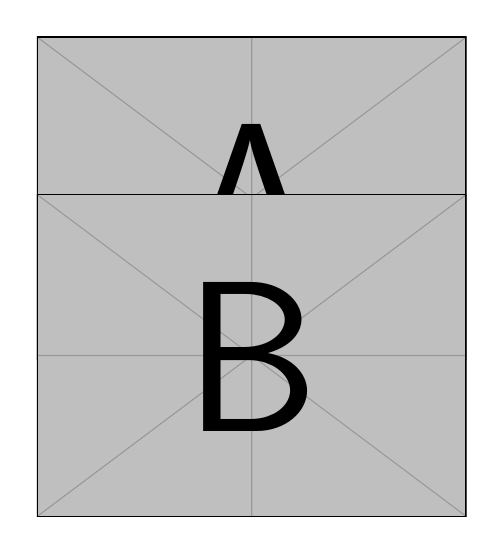
\begin{tikzpicture}[baseline=(current bounding box.north)]
        \node[anchor=north] (pic1) at (0,0) {\includegraphics[width=0.45\textwidth]{example-image-a}};
        \node[anchor=north] (pic2) at (0,-2cm) {\includegraphics[width=0.45\textwidth]{example-image-b}};
    \end{tikzpicture}
\end{table}

\end{document}